\subsection{Classification with AlexNet}
First, we considered the AlexNet classifier pre-trained on ImageNet and tested on the ImageNet subset in its original, black and white and re-colorized versions.

\begin{table*}[ht]
	\begin{center}
		\begin{adjustwidth}{-1cm}{}
			\begin{tabular}{c|ccccccccc}
				&\textbf{Original} & \textbf{B\&W} & \textbf{Baseline w/c}&\textbf{Baseline} & \textbf{Dahl} & \textbf{Zhang} & \textbf{Siggraph} & \textbf{ChromaGAN} & \textbf{InstColorization}  \\
				\midrule
				\textbf{Pre-trained} & 74.5\% & 43.1\% & 32.5\% & 34.0\% & 39.8\% & 42.7\% & 43.2\% & 46.8\% & 49.5\% \\
				\midrule
				\textbf{Feature Extraction} & 97.2\% & 84.2\% & 79.4\% & 80.4\% & 87.8\% & 87.6\% &  88.9\%   &  90.2\% &       90.0\% \\
				\midrule
				\textbf{Finetuning} & 99.7\% & 63.0\% & 58.4\% & 63.6\% & 64.4\% & 80.9\% &  79.9\%   &  77.9\% &       73.7\% \\
			\end{tabular}
		\end{adjustwidth}
	\end{center}
	\caption{{\small  Summary of the classification accuracy of Alexnet in three different settings: Alexnet pre-trained on Imagenet, Alexnet feature extraction for the ImageNet subset, AlexNet finetuning for the Birds and Flowers dataset.}}
	\label{tab:pre-trained}
\end{table*}

\begin{figure*}[t]
	\centering
	\captionsetup[subfigure]{labelformat=empty}
	\begin{subfigure}[b]{0.1\textwidth}
		\centering
		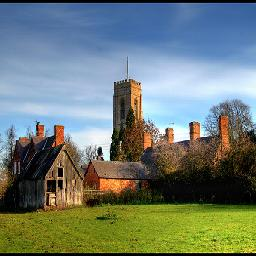
\includegraphics[width=2cm]{or - imgnet.jpeg}
	\end{subfigure}
	\hfill
	\begin{subfigure}[b]{0.1\textwidth}
		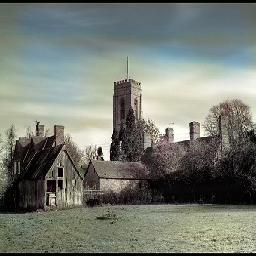
\includegraphics[width=2cm]{b - imgnet.jpeg}
	\end{subfigure}
	\hfill
	\begin{subfigure}[b]{0.1\textwidth}
		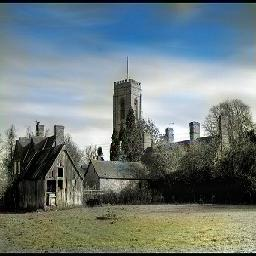
\includegraphics[width=2cm]{bw - imgnet.jpeg}
	\end{subfigure}
	\hfill
	\begin{subfigure}[b]{0.1\textwidth}
		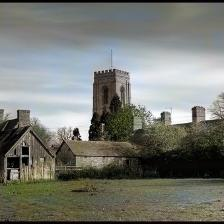
\includegraphics[width=2cm]{d - imgnet.jpeg}
	\end{subfigure}
	\hfill
	\begin{subfigure}[b]{0.1\textwidth}
		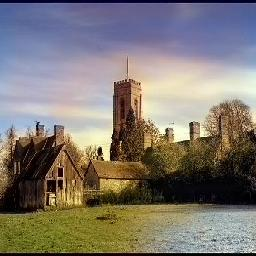
\includegraphics[width=2cm]{z - imgnet2.jpeg}
	\end{subfigure}
	\hfill
	\begin{subfigure}[b]{0.1\textwidth}
		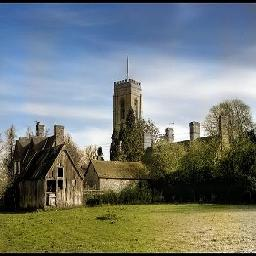
\includegraphics[width=2cm]{si - imgnet2.jpeg}
	\end{subfigure}
	\hfill
	\begin{subfigure}[b]{0.1\textwidth}
		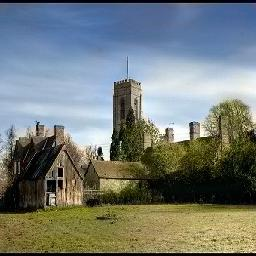
\includegraphics[width=2cm]{chr - imgnet2.jpeg}
	\end{subfigure}
	\hfill
	\begin{subfigure}[b]{0.1\textwidth}
		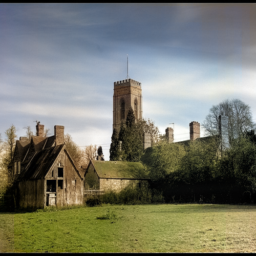
\includegraphics[width=2cm]{su - imgnet.png}
	\end{subfigure}

	\vspace{0.1cm}
	\begin{subfigure}[b]{0.1\textwidth}
		\centering
		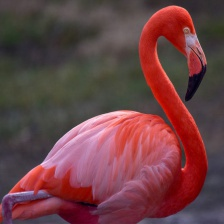
\includegraphics[width=2cm]{or - flamingo.jpg}
		\caption{Original}
	\end{subfigure}
	\hfill
	\begin{subfigure}[b]{0.1\textwidth}
		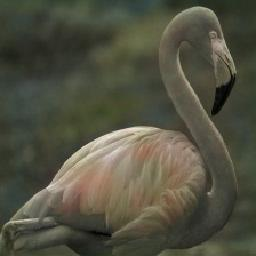
\includegraphics[width=2cm]{bw - flamingo.jpg}
		\caption{Baseline w/c}
	\end{subfigure}
	\hfill
	\begin{subfigure}[b]{0.1\textwidth}
		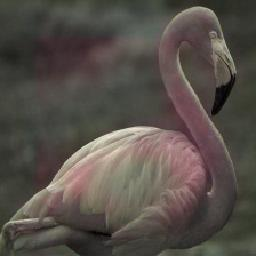
\includegraphics[width=2cm]{b - flamingo.jpg}
		\caption{Baseline}
	\end{subfigure}
	\hfill
	\begin{subfigure}[b]{0.1\textwidth}
		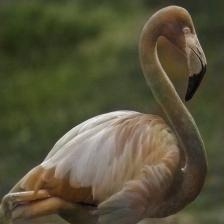
\includegraphics[width=2cm]{d - flamingo.jpg}
		\caption{Dahl}
	\end{subfigure}
	\hfill
	\begin{subfigure}[b]{0.1\textwidth}
		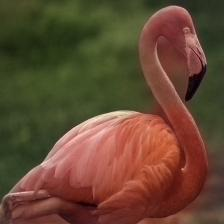
\includegraphics[width=2cm]{z - flamingo.jpg}
		\caption{Zhang}
	\end{subfigure}
	\hfill
	\begin{subfigure}[b]{0.1\textwidth}
		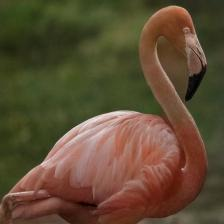
\includegraphics[width=2cm]{si- flamingo.jpg}
		\caption{Siggraph}
	\end{subfigure}
	\hfill
	\begin{subfigure}[b]{0.1\textwidth}
		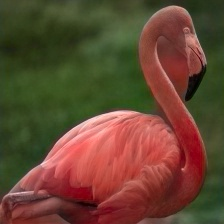
\includegraphics[width=2cm]{chr - flamingo.jpg}
		\caption{ChromaGAN}
	\end{subfigure}
	\hfill
	\begin{subfigure}[b]{0.1\textwidth}
		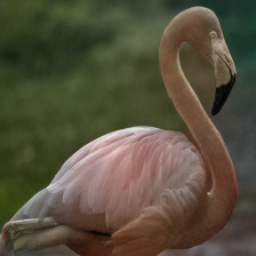
\includegraphics[width=2cm]{su - flamingo.png}
		\caption{InstColoriz.}
	\end{subfigure}
	\caption{{\small Colorization comparison on two images from ImageNet Church (first row) and 325 Birds Species Flamingo (second row).}}
	\label{fig:imagenet}
\end{figure*}

Table \ref{tab:pre-trained} reports the AlexNet classification accuracy in this setting and in other two settings that we will discuss later in this section. Note that the Baseline without cartoonization (Baseline w/c) always reaches a slightly worse accuracy than the Baseline combined with cartoonization, meaning that our approach is valid and can actually improve the colorization performance.

The great gap in the accuracies computed on the original and the black and white versions of the images suggests that colors play an important role in image classification.

The best colorizations according to this experiment are given by ChromaGAN and InstColorization, while the Baseline and Dahl are not even able to improve the accuracy with respect to the black and white images.\\

Overall, the accuracy on the models' colorizations is much lower than the one computed on the original images and the latter is relatively low. Therefore we applied feature extraction to better focus on our ImageNet subset: we used the pre-trained AlexNet as a fixed feature-extractor, and only updated the final layer (for 2 epochs) in order to consider just our 12 ImageNet classes. This resulted in more reliable accuracy values and all the models except the Baseline are able to outperform the black and white images.\\

For a further comparison, we applied finetuning to perform classification on the birds and flowers images, which present more vibrant and various colors than our ImageNet subset: we updated (for 2 epochs) all the AlexNet parameters for the new task. In this new setting we have, as expected, a greater gap than before between the original and the black and white accuracies, meaning that the color is much more relevant. Indeed, all the models including the Baseline with cartoonization are able to improve the accuracy with respect to the black and white images.

The best colorizations according to this experiment are given by the Zhang and Siggraph models, which are able to generalize better across different datasets.

In this last setting, we can notice a general decreasing in the accuracy (except for the original images) with respect to the feature extraction using the ImageNet subset. This is due to the fact that our pre-trained models have been trained on Image-Net and their colorization of the birds and flowers images are overall bad. However, looking at our results, a badly colored image generally seems more distinguishable than its black and white version.

To conclude, the colorizations of two images are reported as an example in Figure \ref{fig:imagenet}.

